\chapter{Experiments: Application of Neural DA to Spectral Data}
\label{exp_chapter}

\section{Data Preparation}

The SDSS DR14 Optical Spectra Catalog contains 4\,851\,200 spectra
and the corresponding SDSS DR14 QSO Catalog contains 526\,356 object.
To the 526\,356 QSO there is supposed to be 649\,791 spectra
according to the QSO catalog metadata.
However, there is a bug in the catalog as some spectra of QSO cannot be identified.
Therefore, we are able to get only 629\,512 spectra of all QSOs
missing 20\,279 spectra of QSOs due to the bug.

Moreover, after cross-matching the general and QSO catalog,
we were unable to find 55 spectra.
Afterall, we end up with correctly identified 629\,457 spectra of QSO.

The labels are incomplete and there will be spectra truly QSO
but not identified in our dataset
acting againt our objective during learning.
We hope to find a robust solution.

LAMOST DR5 General Catalog contains 9\,026\,365 spectra
and its catalog of all QSOs found so far has 42\,552 spectra of QSOs.
However, we were able to cross-match only 31\,755 spectra of QSOs with the general catalog.

\begin{table}
	\begin{center}
	\begin{tabular}{|l|r|r|}
		\hline
		Name & QSOs & Total spectra \\ \hline \hline
		SDSS DR14 & 627\,508 & 4\,816\,713 \\ \hline
		SDSS training set & 130\,904 & 1\,000\,000 \\ \hline
		SDSS validation set & 6\,552 & 50\,000 \\ \hline
		LAMOST DR5 v3 & 31\,755 & 9\,026\,365 \\ \hline
		LAMOST training set & 3\,517 & 1\,000\,000 \\ \hline
		LAMOST validation set & 190 & 50\,000 \\ \hline
	\end{tabular}
	\end{center}
	\caption{Size of data}
\end{table}

Moreover, evaluation on LAMOST data can be biased
because the QSO identification strategy is different in LAMOST and SDSS.
Therefore, some QSO might not be identified in LAMOST.

For neural network training,
we need to have all spectra in the same wavelength range
and measured in the same wavelenghts.
The wavelenght grid is same for both archive.
The grid is in logarithmic wavalength with 0.0001 spacing.
Our aim is to find QSO in the LAMOST archive.
Therefore, we would like to keep as many spectra as possible from the LAMOST archive.
Figure~\ref{wavemin_wavemax_hist} show historgram of minimal and maximal wavelengths of all LAMOST spectra.
The maximum from minimal wavelengths 3\,839.7244 \AA{}
and the minimum from maximal wavelengths 8\,914.597 \AA{}.

\begin{figure}
	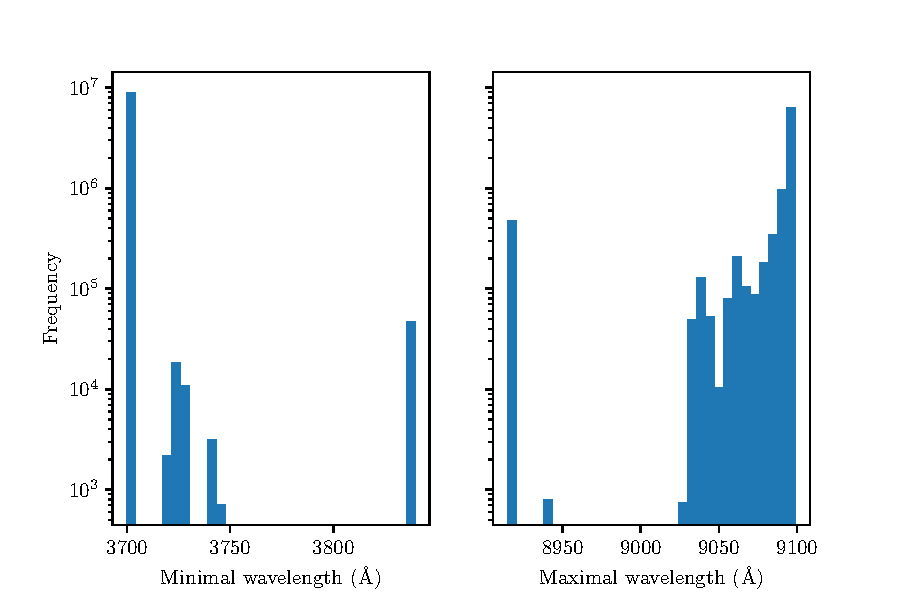
\includegraphics[width=\textwidth]{img/wavemin_wavemax_hist.pdf}
	\caption{Minimal and maximal wavelength of LAMOST spectra}
	\label{wavemin_wavemax_hist}
\end{figure}

\begin{figure}
	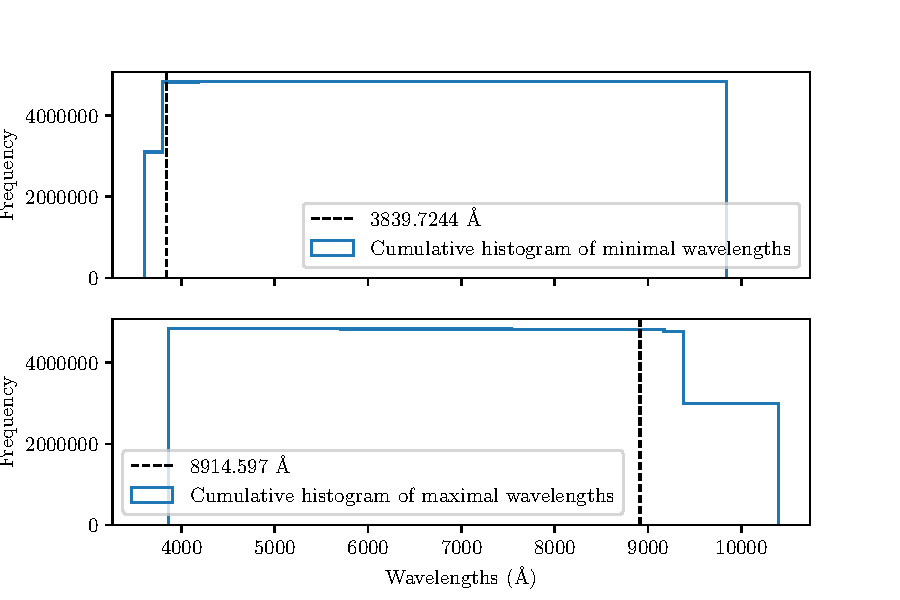
\includegraphics[width=\textwidth]{img/waves_cumulative_hist.pdf}
	\caption{Cutting SDSS specta}
	\label{wavemin_wavemax_hist}
\end{figure}

Min-max preprocessing in the \([-1; 1]\) range:

\begin{equation}
	\mathbf{x}_i = 2 \frac{\mathbf{x}_i - \min(\mathbf{x}_i)}{
		\max(\mathbf{x}_i) - \min(\mathbf{x}_i)} - 1.
\end{equation}

\section{Dimensionality Reduction}

\subsection{Principal Component Analysis (PCA)}

\subsection{t-distributed Stochastic Neighbor Embedding (t-SNE)}

\subsection{Uniform Manifold Approximation and Projection (UMAP)}

\section{Baseline: Results without Use of Deep DA}

LeNet-5 and DeCAF.

\begin{figure}
	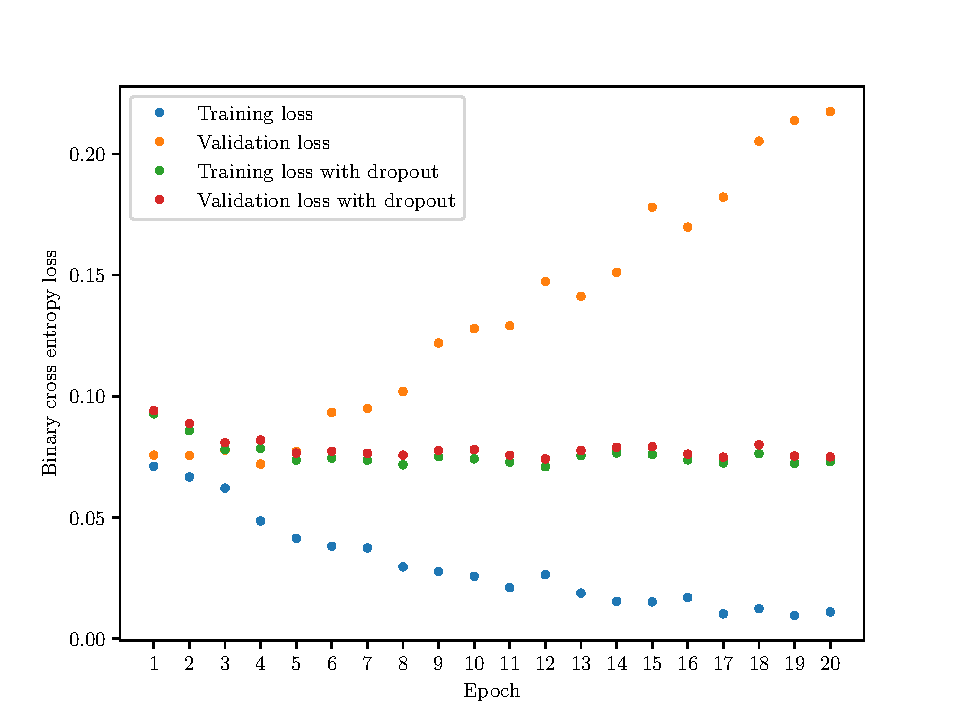
\includegraphics[width=\textwidth]{img/lenet_losses.pdf}
	\caption{Losses of LeNet-5}
	\label{lenet_losses}
\end{figure}

\tikzstyle{layer} = [align=center,draw=black,font=\tiny,rectangle,text centered]
\begin{figure}
\begin{center}
\subfloat[][LeNet-5]{
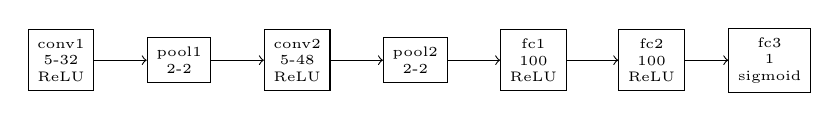
\begin{tikzpicture}[node distance=1.5cm]
	\node (conv1) [layer] {conv1\\5-32\\ReLU};
	\node (pool1) [layer,right of=conv1] {pool1\\2-2};
	\node (conv2) [layer,right of=pool1] {conv2\\5-48\\ReLU};
	\node (pool2) [layer,right of=conv2] {pool2\\2-2};
	\node (fc1) [layer,right of=pool2] {fc1\\100\\ReLU};
	\node (fc2) [layer,right of=fc1] {fc2\\100\\ReLU};
	\node (fc3) [layer,right of=fc2] {fc3\\1\\sigmoid};
	\draw [->] (conv1) -- (pool1);
	\draw [->] (pool1) -- (conv2);
	\draw [->] (conv2) -- (pool2);
	\draw [->] (pool2) -- (fc1);
	\draw [->] (fc1) -- (fc2);
	\draw [->] (fc2) -- (fc3);
\end{tikzpicture}
}\\
\subfloat[][DDC]{
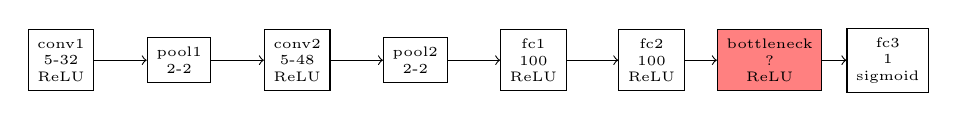
\begin{tikzpicture}[node distance=1.5cm]
	\node (conv1) [layer] {conv1\\5-32\\ReLU};
	\node (pool1) [layer,right of=conv1] {pool1\\2-2};
	\node (conv2) [layer,right of=pool1] {conv2\\5-48\\ReLU};
	\node (pool2) [layer,right of=conv2] {pool2\\2-2};
	\node (fc1) [layer,right of=pool2] {fc1\\100\\ReLU};
	\node (fc2) [layer,right of=fc1] {fc2\\100\\ReLU};
	\node (bottleneck) [layer,right of=fc2,fill=red!50] {bottleneck\\?\\ReLU};
	\node (fc3) [layer,right of=bottleneck] {fc3\\1\\sigmoid};
	\draw [->] (conv1) -- (pool1);
	\draw [->] (pool1) -- (conv2);
	\draw [->] (conv2) -- (pool2);
	\draw [->] (pool2) -- (fc1);
	\draw [->] (fc1) -- (fc2);
	\draw [->] (fc2) -- (bottleneck);
	\draw [->] (bottleneck) -- (fc3);
\end{tikzpicture}
}\\
\subfloat[][DANN]{
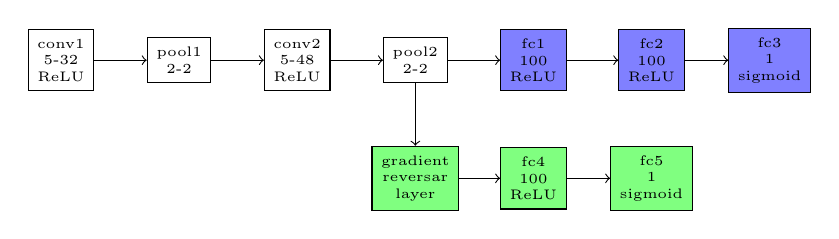
\begin{tikzpicture}[node distance=1.5cm]
	\node (conv1) [layer] {conv1\\5-32\\ReLU};
	\node (pool1) [layer,right of=conv1] {pool1\\2-2};
	\node (conv2) [layer,right of=pool1] {conv2\\5-48\\ReLU};
	\node (pool2) [layer,right of=conv2] {pool2\\2-2};
	\node (fc1) [layer,right of=pool2,fill=blue!50] {fc1\\100\\ReLU};
	\node (fc2) [layer,right of=fc1,fill=blue!50] {fc2\\100\\ReLU};
	\node (fc3) [layer,right of=fc2,fill=blue!50] {fc3\\1\\sigmoid};
	\node (grl) [layer,below of=pool2,fill=green!50] {gradient\\reversar\\layer};
	\node (fc4) [layer,right of=grl,fill=green!50] {fc4\\100\\ReLU};
	\node (fc5) [layer,right of=fc4,fill=green!50] {fc5\\1\\sigmoid};
	\draw [->] (conv1) -- (pool1);
	\draw [->] (pool1) -- (conv2);
	\draw [->] (conv2) -- (pool2);
	\draw [->] (pool2) -- (fc1);
	\draw [->] (fc1) -- (fc2);
	\draw [->] (fc2) -- (fc3);
	\draw [->] (pool2) -- (grl);
	\draw [->] (grl) -- (fc4);
	\draw [->] (fc4) -- (fc5);
\end{tikzpicture}
}\\
\subfloat[][DRCN]{
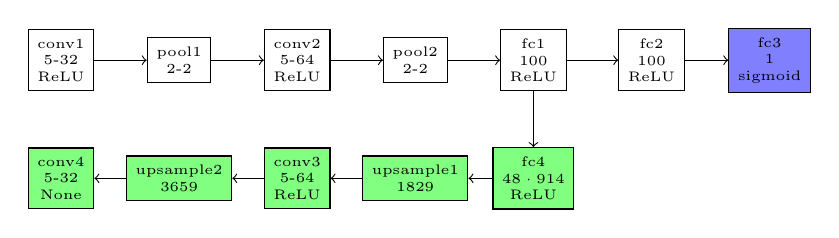
\begin{tikzpicture}[node distance=1.5cm]
	% encoder
	\node (conv1) [layer] {conv1\\5-32\\ReLU};
	\node (pool1) [layer,right of=conv1] {pool1\\2-2};
	\node (conv2) [layer,right of=pool1] {conv2\\5-64\\ReLU};
	\node (pool2) [layer,right of=conv2] {pool2\\2-2};
	\node (fc1) [layer,right of=pool2] {fc1\\100\\ReLU};
	% feature labelling
	\node (fc2) [layer,right of=fc1] {fc2\\100\\ReLU};
	\node (fc3) [layer,right of=fc2,fill=blue!50] {fc3\\1\\sigmoid};
	% decoder
	\node (fc4) [layer,below of=fc1,fill=green!50] {fc4\\\(48 \cdot 914\)\\ReLU};
	\node (upsample1) [layer,left of=fc4,fill=green!50] {upsample1\\1829};
	\node (conv3) [layer,left of=upsample1,fill=green!50] {conv3\\5-64\\ReLU};
	\node (upsample2) [layer,left of=conv3,fill=green!50] {upsample2\\3659};
	\node (conv4) [layer,left of=upsample2,fill=green!50] {conv4\\5-32\\None};
	% connections
	\draw [->] (conv1) -- (pool1);
	\draw [->] (pool1) -- (conv2);
	\draw [->] (conv2) -- (pool2);
	\draw [->] (pool2) -- (fc1);
	\draw [->] (fc1) -- (fc2);
	\draw [->] (fc2) -- (fc3);
	\draw [->] (fc1) -- (fc4);
	\draw [->] (fc4) -- (upsample1);
	\draw [->] (upsample1) -- (conv3);
	\draw [->] (conv3) -- (upsample2);
	\draw [->] (upsample2) -- (conv4);
\end{tikzpicture}
}
\end{center}
\caption{Architectures}
\label{lenet_5}
\end{figure}

\section{Experiments with Deep DA}

Apply domain adaptation to the selected data.

\subsection{DDC: Deep Domain Confusion}

\subsection{DANN: Domain-Adversarial Training of Neural Networks}

\subsection{DRCN: Deep Reconstruction-Classification Networks}

\section{Evaluation of Experiments}

Prepare visualisation of results.
